%%%%%%%%%%%%%%%%%%%%%%%%%%%%%%%%%%%%%%%%%%%%%%%%%%%%%%%%%%%%%%%%%%%%%%%%
%                                                                      %
%     File: Thesis_Implementation.tex                                  %
%     Tex Master: Thesis.tex                                           %
%                                                                      %
%     Author: Andre C. Marta                                           %
%     Last modified :  2 Jul 2015                                      %
%                                                                      %
%%%%%%%%%%%%%%%%%%%%%%%%%%%%%%%%%%%%%%%%%%%%%%%%%%%%%%%%%%%%%%%%%%%%%%%%

\chapter{The \toolname{} Tool}

%%%%%%%%%%%%%%%%%%%%%%%%%%%%%%%%%%%%%%%%%%%%%%%%%%%%%%%%%%%%%%%%%%%%%%%%

\label{solution}
In this chapter we explain in-depth our approach at solving the complex problem of developing a portable static taint analyzer. Our solution, besides being portable, also aims to be able to perform a context-aware analysis.

As stated before, static analyzers are most often bound to a single language and depend on every detail of that language. However, there are a lot of similarities between programming languages, and our approach explores just that. If we take a look at the top trending languages in 2020, ranked by IEEE Spectrum \cite{cass2020top}, used to build web applications, we can divide them in two categories:

\begin{enumerate}
    \item Dynamically typed - Languages that do not check or enforce type-safety at compile-time \cite{tratt2009dynamically}. Instead, type-checking is done during runtime (e.g., Python, JavaScript, PHP and Ruby).
    \item Statically typed - Type checking is done at compile-time (e.g., Java, C\#, GO and Dart).
\end{enumerate}


The languages from each category have many similarities between them. Take for instance JavaScript and PHP, which are very common on web applications. Both of them are object-oriented, have methods, functions, attributes, variables, expressions, etc... Even the \textit{control flow statements} are practically the same (e.g., \textit{if, switch, while, for, do while} etc.). Furthermore, the data flow is almost identical, using assignments. 

Now, if we compare Java and C\# the same is true. Moreover, even comparing languages between categories (e.g., Java and PHP) we see that many of their features overlap. The main difference is that we know the types when analyzing the source code. So from our studies, we found out that when it comes to static taint analysis, we can abstract almost any web programming language. 

With this in mind, our approach introduces a new way of building static analyzers, which consists of having a simple, generic AST (\astname{}) that can represent the structure of the source code of a large set of languages found in web applications. The \astname{}, similarly to the micro-grammars approach \cite{microgrammars}, does not depend on every detail of the languages. Instead, it only represents what is absolutely needed to perform a data flow analysis (in our case, static taint analysis). Section \ref{genericast} explains the abstractions that were made to build the \astname{}.

With the addition of the \astname{}, our analysis gains an extra step comparing to traditional tools. Usually, analyzing a program consists of first parsing the source code and then traversing the resulting AST to find vulnerabilities. By contrast, our approach adds a new, additional step, which consists of converting the source code AST to a \astname{}. Then, we perform the taint analysis on the \astname{} to detect vulnerabilities in the code. This way, the module that performs the taint analysis is completely independent of the language being analyzed. 

Next, we describe the architecture and data flow of \toolname{}. Then, we present the  structure of the \astname{} and how to build it. Finally, we discuss the features of our taint analysis and the compromises and choices that were made.


\section{Architecture and Data Flow}
\label{architecture}


In order to implement a tool that can support several languages simultaneously, we need a decoupled and modular architecture. The architecture of our tool, represented in figure \ref{architecture}, consists mainly of four modules: \textit{Parser}, \textit{AST Converter}, \textit{\astname{} Builder} and \textit{Taint Analyzer}.

\subsection{Parser} 

This module takes as input the source code and produces a source code AST, specific to the language. This module is language-dependent, meaning that every time we add a new language, we need a new parser for that language. Since parsing a full-blown language is a complex task, we delegate it to ANTLR4, which is a widely used parser generator that uses \textit{LL} for parsing \cite{antlr4book}. ANTRL4 has a big community and provides grammars under the MIT license for virtually any language. This way, thanks to ANTRL4, our parsers consist simply of generated code. Furthermore, ANTRL4 also generates tree walkers, which we use to traverse the AST.

\subsection{AST Converter}
Module responsible for traversing the source code AST using the generated tree walker and raising events to the \textit{\astname{} Builder} (e.g., entering and exiting class, methods or functions declarations). These events allow the \textit{\astname{} Builder} to create the \astname{}. This module is the only one needed to program whenever adding support for a new language.

\subsection{\astname{} Builder} 

Module that reacts to the events from the \textit{AST Converter} and internally builds the \astname{}. Section \ref{buildgenericast} shows more in-depth the process of building the \astname{}. 

\subsection{Taint Analyzer} 
Module that takes as input the \astname{} from the \textit{\astname{} Builder} and a configuration file. Then, it traverses the \astname{} using a visitor and propagates the taint marks to find vulnerabilities according to the configuration file. 
Listing \ref{settings} shows an example of a configuration file. In this file, we can specify the value of several parameters, such as:
\begin{itemize}
    \item Source code location - we can set the directory where the source code is and the file extensions that we want to analyze (lines 2, 3)
    \item Entry points - the file and the function where the data flow propagation should start. In the example, it corresponds to lines 6-14, where the entry point is a function called \textit{functionEntryPoint} from the class \textit{EntryPointClass} in the file \textit{EntryPointClass.java}. We also specify which arguments are \textit{tainted}: \textit{"taintedArg","userInput"}
    \item Sensitive sinks - functions that when called with \textit{tainted} arguments may result in a vulnerability. In the example we specify a function named \textit{executeQuery} from the class \textit{Statement} (lines 15-26). For each sensitive function we can set a list of functions that can sanitize its inputs. A sanitization function is a function that cleans the input from malicious characters and whose return value is always \textit{untainted} (e.g., one sanitization function for \textit{mysql\_query} is \textit{mysqli\_real\_escape\_string}). In listing \ref{settings} we configure a sanitization method called \textit{sanitizeInputMethod} from the class \textit{SanitizerClass}. This mapping between sensitive and sanitization functions allows us precisely specify the correct sanitization function for each sensitive function, thus reducing false negatives in our analysis.
    
    \item Loops settings - number of times we should analyze a loop. We explain this choice more in-depth in section \ref{loops}.
\end{itemize}


\begin{lstlisting}[
    showstringspaces=false,
    caption={Example of file settings},
    label=settings, float]
{
    "directoryPath": "path/to/app",
    "fileExtension": ".java",
    "numberOfTimesToAnalyzeCycles" : 2,
    "specification": {
        "filename": "EntryPointClass.java",
        "function": {
            "name": "functionEntryPoint",
            "type": "EntryPointClass"
        },
        "taintedVarsOrArgs": [
            "taintedArg",
            "userInput"
        ],
        "sensitiveFunctions": [
            {
                "name": "exectuteQuery",
                "type": "Statement",
                "sanitizationFunctions": [
                    {
                        "name": "sanitizeInputMethod",
                        "type": "SanitizerClass"
                    }
                ]
            }
        ],
        "returnTaintedIfTaintedSource": true,
        "taintedAttributes": [
            "taitedAttributeName"
        ]
    }
}
\end{lstlisting}


After traversing the \astname{}, \toolname{} produces a vulnerability report in JSON format. Listing \ref{report} shows an example of a report when analyzing listing \ref{pathpropagation}. In the report, \toolname{} presents the vulnerabilities and the time that took to analyze the program. Furthermore, for each vulnerability it presents a list of conditions that need to be met to reproduce the vulnerability. 

\begin{lstlisting}[
    showstringspaces=false,
    caption={Vulnerability report when analyzing listing \ref{pathpropagation}},
    label=report, float]
{
    "vulnerabilities": [
        {
            "file": "EntryPointClass.java",
            "line": 7,
            "vulnerableMethod": "executeQuery",
            "functionCallStack": [],
            "conditions": [
                {
                    "line": 2,
                    "condition": "input != null"
                },
            ]
        }
    ],
    "timeToProcessMilliseconds": 2074
}
\end{lstlisting}


\begin{figure}[hbt!]
    \centering
    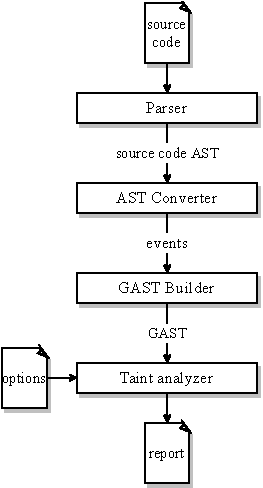
\includegraphics[width =0.4\linewidth]{images/yasat-architecture.pdf}
    \caption{\toolname{} - data flow and architecture overview} 
    \label{architecture}
\end{figure}

\section{\astname{}}
\label{genericast}
Similarly to the micro-grammars solution \cite{microgrammars}, the \astname{} aims to be an intermediate structure that does not depend on every detail of any language. Instead, it abstracts most of the complexity by using generic statements. Each generic statement has a correspondence with a concrete statement of almost any programming language. In this section we describe the structure of the \astname{} by presenting every element that can be part of it. 

\subsection{Elements}

\subsubsection{Constant} 
Element that comprises \textit{strings}, \textit{integers}, \textit{floats}, \textit{null} values etc. Basically, everything that is directly hardcoded in the source code is considered a constant. Since this element never changes, it is impossible to be \textit{tainted}. Figure \ref{constant} presents the \astname{} representation of a constant.

\begin{figure}[hbt!]
    \centering
    \begin{forest}
        [Constant [\textit{value}] ]
    \end{forest}  
    \caption{\astname{} representation of a constant}\label{constant}
\end{figure}


 
\subsubsection{Variable}

This element abstracts, as the name says, the variables in the code. Contains the name of the variable, and if the language is statically typed, it also contains the type of the variable. It can become \textit{tainted} through assignments. Figure \ref{variable} shows the \astname{} representation of a variable.

\begin{figure}[hbt!]
    \centering
    \begin{forest}
        [Variable 
            [\textit{name}]
            [\textit{type}]
        ]
    \end{forest}  
    \caption{\astname{} representation of a variable}\label{variable}
\end{figure}


\subsubsection{Attribute} 
Represents an attribute in a class. It has a name and a type. Also, it can be \textit{tainted}. It is very similar to a variable, as we can see in its representation from figure \ref{attribute}. In our implementation an attribute is a subtype of \textit{Variable}.

\begin{figure}[hbt!]
    \centering
    \begin{forest}
        [Attribute 
            [\textit{name}]
            [\textit{type}]
        ]
    \end{forest}  
    \caption{\astname{} representation of an attribute}\label{attribute}
\end{figure}

\subsubsection{Parameter} Element that abstracts the parameters of methods and functions. It can be \textit{tainted} if it is the parameter of the entry point function, or if the argument passed to a function is \textit{tainted}. Just like the \textit{attribute}, it is also a subtype of \textit{variable}. Figure \ref{parameter} presents its \astname{} representation. 

\begin{figure}[hbt!]
    \centering
    \begin{forest}
        [Parameter 
            [\textit{name}]
            [\textit{type}]
        ]
    \end{forest}  
    \caption{\astname{} representation of a parameter}\label{parameter}
\end{figure}

\subsubsection{Expression} 
Represents a generic abstraction of any expression (e.g., arithmetic, logical, bitwise, comparison etc.). It consists of a list of expressions.
Take for instance the listing \ref{javaexpression} where to each variable, \textit{a, b, c} we assign an expression. In our representation, all these expressions are equal. They all consist of an expression containing two members: a variable named \textit{"x"} and a constant with value \textit{"5"}. This allows us to abstract any operator due to the fact that in data flow analysis, operators (except the assignment operators) do not influence \textit{taint} propagation. For instance, if the variable \textit{x} in listing \ref{javaexpression} is \textit{tainted}, then, all variables will be \textit{tainted}, regardless of their operator.

\begin{lstlisting}[language=Java,
    showstringspaces=false,
    caption={Expression assignment examples},
    label=javaexpression]
boolean a = x == 5;
int b = x + 5;
int c = x * 5;
\end{lstlisting}


\begin{figure}[hbt!]
    \centering
    \begin{forest}
        [Expression 
            [\textit{members}
                [Variable 
                    [\textit{name} [x]]
                    [\textit{type} [int]]
                    ]
                [Constant [\textit{value} [5]]]
            ]
        ]
    \end{forest}  
    \caption{\astname{} representation of the expressions from listing \ref{javaexpression}}\label{expression}
\end{figure}


Since an expression consists only of a list of other expressions, the \textit{taint} propagation is a result of a logical OR of all elements in the expression. Meaning that if any element in the list is \textit{tainted}, the whole expression is marked as \textit{tainted}. 





\subsubsection{Function Call} This element is a subtype of \textit{expression} with the difference that it has a name, referencing the function it is invoking. The arguments are just a list of expressions that can contain anything. Figure \ref{funccall} shows the \astname{} representation of a function call.

\begin{figure}[hbt!]
    \centering
    \begin{forest}
        [Function Call 
            [\textit{name}]
            [\textit{members}]
        ]
    \end{forest}  
    \caption{\astname{} representation of a function call}\label{funccall}
\end{figure}

For instance, the function call \textit{executeQuery(getQuery("name"))} is named \textit{executeQuery} and has as argument another function call named \textit{getQuery}. The latter having as argument a constant with value \textit{"name"}. Figure \ref{funccall1} represents the described tree.

\begin{figure}[hbt!]
    \centering
    \begin{forest}
        [Function Call 
            [\textit{name} [executeQuery]]
            [\textit{members} 
                [Function Call 
                    [\textit{name} [getQuery] ]
                    [Constant [\textit{value} [name]]]
                ]
            ]
        ]
    \end{forest}  
    \caption{\astname{} representation of \textit{"executeQuery(getQuery("name")"}}\label{funccall1}
\end{figure}


A function call is considered \textit{tainted} if any of the following conditions is true: 
\begin{itemize}
    \item the called function is in the source code and it returns a \textit{tainted} value
    \item the called function is in a library and any of its arguments is \textit{tainted}
\end{itemize}

This element also represents method calls that do not have an object as a source (e.g., methods from the same class or any superclass that are not preceded by the keywords \textit{this} or \textit{super} in Java).

\subsubsection{Assignment} 
Statement that represents, as the name indicates, an assignment. Consists of two expressions, one on the left-hand side and another on the right-hand side. It is the main way of propagating \textit{taint} marks. Whenever the expression assigned on the right is evaluated as \textit{tainted}, the mark is also propagated to the expression on the left. Usually, the expression on the left-hand side is just a variable. Listing \ref{javaexpression} contains examples of assignment statements and figure \ref{assignment} shows the \astname{} representation of an assignment.


\begin{figure}[hbt!]
    \centering
    \begin{forest}
        [Assignment
            [\textit{left} 
                [Variable 
                    [\textit{name} [a]]
                    [\textit{type} [boolean]]
                ]
            ]
            [\textit{right} 
                [Expression 
                    [\textit{members}
                        [Variable 
                            [\textit{name} [x]]
                            [\textit{type} [int]]
                            ]
                        [Constant [\textit{value} [5]]]
                    ]
                ]
            ]
        ]
    \end{forest}  
    \caption{\astname{} representation of \textit{"boolean a = x == 5;"}}\label{assignment}
\end{figure}

\subsubsection{Return} This statement, represented in figure \ref{return}, represents the end of the data flow in a path. The returned value is represented by an \textit{expression} which can be \textit{tainted}.

\begin{figure}[hbt!]
    \centering
    \begin{forest}
        [Return 
            [\textit{expression}]
        ]
    \end{forest}  
    \caption{\astname{} representation of a return statement}\label{return}
\end{figure}


\subsubsection{Throw} 
Statement very similar to the return statement. The only difference is that when a return statement is found in the callee function, the data flow is transferred to the caller function. Whilst in the case of a throw statement, the data flow is transferred to a catch block. The thrown expression can be \textit{tainted}. Figure \ref{throw} shows the \astname{} representation of the throw statement.  

\begin{figure}[hbt!]
    \centering
    \begin{forest}
        [Throw 
            [\textit{expression}]
        ]
    \end{forest}  
    \caption{\astname{} representation of a throw statement}\label{throw}
\end{figure}



\subsubsection{Method Call}  
Element that represents method calls. It consists of a source, which can be an object or a class (if the method is static). Listing \ref{methodcall} shows examples of method calls where the source is an object and a class respectively. Figure \ref{methodcallex} shows the \astname{} representation of the first example of listing \ref{methodcall}.

\begin{lstlisting}[language=Java,
    showstringspaces=false,
    caption={Method call examples},
    label=methodcall, float]
context.getUsers();
MyClass.myStaticMethod();
\end{lstlisting}

\begin{figure}[hbt!]
    \centering
    \begin{forest}
        [Method Call
            [\textit{source}
                [Variable 
                    [\textit{name} [context]]
                    [\textit{type} [UserContext]]
                ]
            ]
            [\textit{call} 
                [Function Call
                    [\textit{name} [getUsers]]
                ]
            ]
        ]
    \end{forest}  
    \caption{\astname{} representation of \textit{"context.getUsers();"}}\label{methodcallex}
\end{figure}

A method call is \textit{tainted} if any of the following conditions is true:

\begin{itemize}
    \item the method is not in the analyzed code and the source is \textit{tainted}
    \item the method is in the source code and returns a \textit{tainted} value
\end{itemize}







\subsubsection{New} 
Expression that represents an object creation. It is a subtype of \textit{Expression} and works mostly as a function call to the constructor. Figure \ref{new} shows the \astname{} representation of the \textit{new} expression.

In most languages, the constructor has the same name as the class. But in some languages, the name of the constructor is different from the name of the class (e.g., PHP, Python). For these cases, we keep a configuration file with the names. For instance, \textit{new Foo()} in PHP would result in the call of \textit{\_\_construct()} function of the class \textit{Foo}.

\begin{figure}[hbt!]
    \centering
    \begin{forest}
        [New
            [\textit{name}]
            [\textit{members}]
        ]
    \end{forest}  
    \caption{\astname{} representation of a new expression}\label{new}
\end{figure}


\subsubsection{Attribute access} 
Represents a direct access to an object attribute (e.g., \textit{context.myProperty}). Figure \ref{attributeaccess} shows its \astname{} representation.

\begin{figure}[hbt!]
    \centering
    \begin{forest}
        [Attribute access
            [\textit{source}]
            [\textit{name}]
        ]
    \end{forest}  
    \caption{\astname{} representation of an attribute access}\label{attributeaccess}
\end{figure}



\subsubsection{Code block} 
Element that represents a block of code. Consists of a list of statements. Listing \ref{javaexpression} is an example of a code block with three statements and figure \ref{codeblock} shows the \astname{} of listing \ref{javaexpression}.

\begin{figure}[hbt!]
    \centering
    \begin{forest}
        [Code Block
            [\textit{statements}
                [Assignment
                    [\textit{left} 
                        [Variable 
                            [\textit{name} [a]]
                            [\textit{type} [boolean]]
                        ]
                    ]
                    [\textit{right} 
                        [Expression 
                            [\textit{members}
                                [Variable 
                                    [\textit{name} [x]]
                                    [\textit{type} [int]]
                                    ]
                                [Constant [\textit{value} [5]]]
                            ]
                        ]
                    ]
                ]
                [Assignment,
                    [\textit{left} 
                        [Variable 
                            [\textit{name} [b]]
                            [\textit{type} [int]]
                        ]
                    ]
                    [\textit{right} 
                        [...]
                    ]
                ]
                [Assignment
                    [\textit{left} 
                        [Variable 
                            [\textit{name} [c]]
                            [\textit{type} [int]]
                        ]
                    ]
                    [\textit{right} 
                        [...]
                    ]
                ]  
            ]
        ]
    \end{forest}  
    \caption{\astname{} representation of the code block from listing \ref{javaexpression}}\label{codeblock}
\end{figure}



\subsubsection{Conditional statement} 

Element that abstracts loops (e.g., \textit{for, while, do while} etc.). Consists of a code block and a condition, which is an expression. Figure \ref{condstatement} shows its \astname{} representation. 


\begin{figure}[hbt!]
    \centering
    \begin{forest}
        [Conditional statement
            [\textit{expression}]
            [\textit{code block}]
        ]
    \end{forest}  
    \caption{\astname{} representation of a conditional statement}\label{condstatement}
\end{figure}


\subsubsection{Try Catch} 
Statement composed of a \textit{try} code block, a list of \textit{catch} code blocks and one \textit{finally} code block.
Figure \ref{trycatch} shows its \astname{} representation.



\begin{figure}[hbt!]
    \centering
    \begin{forest}
        [Try Catch
            [\textit{try} [Code Block]]
            [\textit{catch} 
                [Code Block]
                [...]
            ]
            [\textit{finally}[Code Block]]
        ]
    \end{forest}  
    \caption{\astname{} representation of a try catch statement}\label{trycatch}
\end{figure}


\subsubsection{If} Statement that abstracts control flow statements (e.g., \textit{if-else, if-elseif-else} and \textit{switch}). Each option in the control flow has its own code block (e.g., \textit{if-else} has two code blocks - one for \textit{if} and another for the \textit{else}). Figure \ref{ifstmt} shows its \astname{} representation.


\begin{figure}[hbt!]
    \centering
    \begin{forest}
        [If Statement
            [\textit{expression}]
            [\textit{code block}]
            [\textit{else ifs} 
                [If Statement]
                [...]
            ]
            [\textit{else}]
        ]
    \end{forest}  
    \caption{\astname{} representation of an if statement}\label{ifstmt}
\end{figure}

\subsubsection{Function} 
Element that represents a method or a function. It has a name, a return type, a list of parameters and a code block. Its representation can be seen in figure \ref{function}.

\begin{figure}[hbt!]
    \centering
    \begin{forest}
        [Function
            [\textit{name}]
            [\textit{return type}]
            [\textit{parameters} 
                [Parameter]
                [...]
            ]
            [\textit{code block}]
        ]
    \end{forest}  
    \caption{\astname{} representation of a function}\label{function}
\end{figure}


\subsubsection{Class}
This element represents a class in the \astname{}. It has a name, a list of attributes and a list of methods. Furthermore, it can have a superclass, as shown in figure \ref{class}.

\begin{figure}[hbt!]
    \centering
    \begin{forest}
        [Class
            [\textit{name}]
            [\textit{superclass}]
            [\textit{attributes} 
                [Attribute]
                [...]
            ]
            [\textit{methods} 
                [Function]
                [...]
            ]
        ]
    \end{forest}  
    \caption{\astname{} representation of a class}\label{class}
\end{figure}


\subsubsection{File} 
This is the root element of any \astname{}. It has a code block (for languages like PHP or JavaScript), a list of classes, a list of functions and a list of imported files (used to trace calls to imported function). Its structure is represented in figure \ref{file}


\begin{figure}[hbt!]
    \centering
    \begin{forest}
        [File
            [\textit{name}]
            [\textit{code block}]
            [\textit{classes} 
                [Class]
                [...]
            ]
            [\textit{imported files} 
                [File]
                [...]
            ]
        ]
    \end{forest}  
    \caption{\astname{} representation of a file}\label{file}
\end{figure}



One important note to keep in mind is that not every language will use every feature from the \astname{}. For instance, the file element can have statements directly in the root block. Now, this is a feature that it is only used by languages such as PHP and JavaScript. By contrast, Java and C\# do not allow code outside classes, so they do not make use of this feature. 

\subsection{Structure}
As an example of the structure of the \astname{}, consider listings \ref{sametreephp} and \ref{sametreejava}. These listings present code with the exact same functionality written in two different languages (Java and PHP). The code is quite simple -- a class with a method that executes an SQL query given an id. 
Parsing both listings with traditional parsers would result in quite different ASTs, despite the code being very similar. However, when converting the source code ASTs to \astname{}, their representation is almost identical. Figure \ref{sametree} represents the \astname{} from listings \ref{sametreejava} and \ref{sametreephp} where the circled branches only appear in the Java representation since it is statically typed.


\begin{lstlisting}[
        language=php,
        showstringspaces=false,
        caption={MyDbClass in PHP},
        label=sametreephp, float] 
class MyDbClass
{
    function getAddressById($id)
    {
        $sql = "SELECT address FROM users WHERE id = $id";
        return executeSQLQuery($sql);
    }
}
\end{lstlisting}
    
    
\begin{lstlisting}[
    language=Java,
    showstringspaces=false,
    caption={MyDbClass in Java},
    label=sametreejava, float]
public class MyDbClass
{
    public static String getAddressById(String id)
    {
        String sql = "SELECT address FROM users WHERE id =" + id;
        return executeSQLQuery(sql);
    }
}
\end{lstlisting}


    
\begin{figure}[hbt!]
    \begin{forest}
        [File
            [\textit{classes}
                [Class
                    [\textit{methods}
                        [Function
                            [\textit{name}[executeSQLQuery]]
                            [\textit{parameters}
                                [Parameter
                                    [\textit{name}[id]]
                                    [\textit{type},tikz={\node[draw,ellipse,black,fit=()(!1),inner sep=0mm]{};} [String]]
                                ]
                            ]
                            [\textit{return type},tikz={\node[draw,ellipse,black,fit=()(!1),inner sep=0mm]{};}[String]]
                            [\textit{code block}
                                [\textit{statements},l*=3
                                    [Assignment 
                                        [\textit{left}
                                            [Variable
                                                [\textit{name}[sql]]
                                                [\textit{type},tikz={\node[draw,ellipse,black,fit=()(!1),inner sep=0mm]{};}[String]]
                                            ]
                                        ]
                                        [\textit{right}
                                            [Expression
                                                [\textit{members}
                                                    [Constant[\textit{value}[{"SELECT address FROM users WHERE id ="}]]]
                                                    [Variable[\textit{name}[id]]]
                                                ]
                                            ]
                                        ]
                                    ]
                                    [Return 
                                        [\textit{expression}
                                            [FunctionCall
                                                [\textit{name}[executeSQLQuery]]
                                                [\textit{members}[Variable[\textit{name}[id]]]]
                                            ]
                                        ]
                                    ]
                                ]
                            ]      
                        ]
                    ]
                    [\textit{name}[MyDbClass]]  
                ]
            ]
            [\textit{name}[MyDbClass.java]]
        ]
    \end{forest}  
    \vspace*{5mm}
    \caption{\astname{} representing the code from listing \ref{sametreejava} and \ref{sametreephp}} 
    \label{sametree}
\end{figure}




\section{Building the \astname{}}
\label{buildgenericast}

In order to build the \astname{}, we first parse the source code using a parser generated by ANTLR4 to obtain the source code AST. Then, we convert the AST to the \astname{} representation. To do this, we use a tree walker also generated by ANTLR4. The tree walker, which conceptually is a visitor, traverses every node of the AST and for each node it invokes a function when it enters or exits that node. So, in order to convert the AST to \astname{} we need to override some of these methods in the \converter{} to pass state to the \textit{\astname{} Builder}. This is due to the fact that the \textit{\astname{} Builder} keeps the current context in a stack and these methods indicate what is the new context to push and when to pop it. This way the \converter{} is just a class that overrides a set of methods from the generated tree walker. 

Listing \ref{funccallconvertexample} shows part of the PHP \converter{}. In the example, we override two methods from the generated tree walker. The first method is invoked when the tree walker enters a \textit{Func} node and the second when it exits the same node. So, when the tree walker reaches a \textit{Func} node, it invokes the method \textit{enterFunc} from the \converter{}. The latter then invokes a method from the \textit{\astname{} Builder} that pushes the function element to the stack. This way, the \textit{\astname{} Builder} is able to keep track of the context. For instance, if the tree walker encounters a \textit{Parameter} node while in the \textit{Func} node, the parameter would be added to the element on the top of the stack, which in this case would be a function. The function is then popped from the stack when tree walker exits the \textit{Func} node, invoking the method \textit{exitFunc} which calls a method from the \textit{\astname{} Builder} that pops the function (line 8). 

\begin{lstlisting}[language=Java,
    showstringspaces=false,
    caption={Function declaration example},
    label=funccallconvertexample, float]
@Override
public void enterFunc(FuncContext ctx) {
    gastBuilder.addFunction(ctx, ctx.name());
}

@Override
public void exitFunc(FuncContext ctx) {
    gastBuilder.exitFunctionOrMethodDeclaration();
}
\end{lstlisting} 

One important note is that we only push to the stack statements (e.g., functions, classes, assignments, conditional statements, etc.), which are nodes in the AST, while elements such as variables, constants or parameters are not pushed. This is due to the fact that they represent leaves in the AST, so they would be pushed and popped right away. This simplification allows us to override less methods from the tree walker when writing the \converter{} (e.g., we do not need to override \textit{exitVariable}).


Let us now consider listing \ref{assignmentconvertexample} where line 1 corresponds to the assignment being built and lines 3-9 to the sequence of calls made by the \converter{} to the \textit{\astname{} Builder}. Due to lack of space, the signatures of the overridden methods are omitted. When the tree walker enters the assignment, the \converter{} calls a method that adds an assignment to the stack (line 3). Next, it enters a variable and since the assignment is on the top of the stack, the variable becomes the left side of the assignment (line 4). Then, the tree walker enters the expression \textit{"x == 5"} and the \converter{} calls a method that adds an expression to the stack (line 5). After that, it enters a variable and later a constant, which will both be added to the expression, since it is the top of the stack (lines 6, 7). Finally, the tree walker first exits the expression and then the assignment, calling \textit{exitStatementOrExpression} twice (lines 8, 9). Figure \ref{assignment} represents the resulting \astname{} and figure \ref{stacks} represents the stack states when building the tree.

\begin{lstlisting}[language=Java,
    showstringspaces=false,
    caption={Assignment build call sequence},
    label=assignmentconvertexample, float]
boolean a = x == 5;

gastBuilder.addAssignment(ctx);
gastBuilder.addVariable(ctx.VarName());
gastBuilder.addExpression(ctx);
gastBuilder.addVariable(ctx.VarName());
gastBuilder.addConstant(ctx.getText());
gastBuilder.exitStatementOrExpression();
gastBuilder.exitStatementOrExpression();
\end{lstlisting}


\begin{figure}[hbt!]
    \subcaptionbox{}[.333\linewidth]
    {\begin{tikzpicture}
        \selectcolormodel{gray}
        \cell[fill=none]{Assign}
        \stacktop[fill=none]{}
    \end{tikzpicture}}
    \subcaptionbox{}[.333\linewidth]
    {\begin{tikzpicture}
        \cell[fill=none]{Assign [Var a]}
        \stacktop[fill=none]{}
      \end{tikzpicture}}      
      \subcaptionbox{}[.333\linewidth]
    {\begin{tikzpicture}
        \cell[fill=none]{Assign [Var a, Expr]}
        \cell[fill=none]{Expr}
        \stacktop[fill=none]{}
    \end{tikzpicture}}
    \subcaptionbox{}[.333\linewidth]
    {\vspace*{5mm}\begin{tikzpicture}
        \cell[fill=none]{Assign [Var a, Expr]}
        \cell[fill=none]{Expr [Var x]}
        \stacktop[fill=none]{}
    \end{tikzpicture}}
    \subcaptionbox{}[.333\linewidth]
    {\vspace*{5mm}\begin{tikzpicture}
        \cell[fill=none]{Assign [Var a, Expr]}
        \cell[fill=none]{Expr [Var x, Const y]}
        \stacktop[fill=none]{}
    \end{tikzpicture}}
    \subcaptionbox{}[0.333\linewidth]
    {\vspace*{5mm}\begin{tikzpicture}
        \cell[fill=none]{Assign [Var a, Expr]}
        \stacktop[fill=none]{}
    \end{tikzpicture}}    

    \vspace{5mm}
    \caption{Stack state when executing code from listing \ref{assignmentconvertexample}}\label{stacks}
\end{figure}


Converting the AST is as simple as identifying the methods needed to override from the generated tree walker, and then call the functions from the \textit{\astname{} Builder}.
For example, the converter for PHP has 67 lines of code (counting only statements), and from these 67 statements, there are 29 that are different, meaning that a lot of the functions invoked are the same (e.g., \textit{exitStatementOrExpression} is invoked 23 times). 


\section{Analysis features}
\label{analysisfeatures}
Our approach is to use a context-aware static taint analysis to find all potential security vulnerabilities. To be able to statically find vulnerabilities, it is necessary to know what \textit{objects} each variable may refer to, a general problem known as \textit{pointer}, \textit{points-to} or \textit{alias analysis}\cite{sridharan2013alias}. Also, the tool must perform a \textit{path aware} \textit{taint} propagation. Furthermore, it must be able to detect function/method calls between different files.

Next, we discuss the importance of the \textit{alias analysis}. Then, we present our solution to a \textit{path aware} analysis and the method \toolname{} uses to find function/method calls from different files. Finally, we describe our approach to handle loops.

\subsection{Pointer information} 
To illustrate the importance of pointer information, consider the example from listing \ref{pointer}. Assume that \textit{param} is tainted and that \textit{executeQuery} is a sensitive function. In this example, a more conservative approach may assume that \textit{buf1} and \textit{buf2} may reference the same object, thus marking both calls to \textit{executeQuery} as tainted. Instead, \toolname{} traces the data flow through assignments made in each execution path. Thus, being able to identify that line 9 is a safe call and line 13 is a vulnerability.


\begin{lstlisting}[
    language=Java,
    showstringspaces=false,
    caption={Taint propagation example},
    label=pointer, float] 
String param = req.getParameter("name");
StringBuffer buf1;
StringBuffer buf2;

...

buf1.append(param);
String query = buf2.toString();
con.executeQuery(query);

buf2 = buf1;
query = buf2.toString();
con.executeQuery(query);
\end{lstlisting}

Pointer analysis has been subject of much compiler research over the last decades \cite{spath2016boomerang,hind2001pointer}. Since determining what heap object a given variable may point to is undecidable, our approach computes only an approximation based on the data flow through assignments. Meaning that, in much more complex cases, when \toolname{} is unsure to which reference an object is pointing to, it assumes that they all point to the same instance.


\subsection{Path Analysis} In order to perform a precise static taint analysis it is very important to be able to track the data through different paths, ideally all of them. However, in practice, it is almost impossible since static path analysis is a very complex problem. The path is often decided at runtime due to features like \texttt{instanceof}, dynamic dispatch or reflection in Java \cite{hammer2008static}. Furthermore, these features differ between languages. Because of this, we can not have the most precise path analysis for each language. Instead, we perform an approximate path analysis based only on the \textit{control flow statements}, ignoring their conditions. This means that we only look at the structure of the code, and for each conditional statement we propagate the data flow twice: one assuming that the flow enters that path and another assuming it does not. This assumption has the disadvantage of propagating \textit{taint} marks through impossible paths.

Consider now the example from listing \ref{pathpropagation} and assume that the variable \textit{input} is \textit{tainted}. Observing the code, we can easily identify an SQL injection vulnerability at line 7, since at line 3 the \textit{query} is concatenated with the \textit{input}.
In this example, \toolname{} propagates the \textit{taint} marks through two paths: the first executing the \textit{if} and the second the \textit{else}. Finally, it reports the vulnerability at line 7. Also, it mentions that this vulnerability only happens if the expression \textit{"input != null"} at line 2 is true. In more complex cases, for each vulnerability \toolname{} returns the call stack and the conditions that need to be met.

\begin{lstlisting}[
    language=Java,
    showstringspaces=false,
    caption={Path propagation example},
    label=pathpropagation, float] 
String query = "SELECT * FROM users WHERE name=";
if (input != null){
    query = query + input;
} else {
    query = query + "Bob";
}
con.executeQuery(query);
\end{lstlisting}

Let us now consider the example from listing \ref{pathpropagation1}. This example is almost identical to listing \ref{pathpropagation}, with the exception of line 2. This assignment makes the instruction from line 4 unreachable, meaning that in practice, the code has only one possible path. However, \toolname{} has exactly the same output as the previous example: two paths and one vulnerability. This is due to the fact that \toolname{}, and static analysis tools in general, struggle with detecting whether a condition can be true or not.

\begin{lstlisting}[
    language=Java,
    showstringspaces=false,
    caption={Path propagation example with unreachable branch},
    label=pathpropagation1] 
String query = "SELECT * FROM users WHERE name=";
input = null;
if (input != null){
    query = query + input;
} else {
    query = query + "Bob";
}
con.executeQuery(query);
\end{lstlisting}

This way, we perform an approximate path analysis based on the \textit{control flow statements} and their code blocks. The advantage of this kind of path detection is that it can be applied to any language. Furthermore, from our testing, most of the times it is enough to detect vulnerabilities, even though it is not the most accurate.


\subsection{Cross-file function referencing} 
In the last decades, web applications have become increasingly more complex, consisting of many files. For this reason, in order to perform a precise static analysis, we need to be able to perform \textit{taint} propagation between files. However, languages have different ways of importing code. For instance, Java imports packages, which consist of a set of classes, and PHP imports files directly \cite{rountev2004static,hills2014static}. 

To mitigate this problem, our approach supports two generic ways of importing code:
\begin{enumerate}
    \item File inclusion - usually used by dynamically typed languages, such as PHP, Python and JavaScript. Each file has a list of imported files. When \toolname{} finds a call to a function that is not found in the file, it searches in all imported files for that function. If more than one is found, it analyses all of them.
    
    \item Type tracking - works for most of the object-oriented languages, such as Java and C\#. Consists of checking the type of the target of the method call and then checking if that class is in the source code. If the class is found it tries to find the method. If the method is not found, it goes to the superclass.
\end{enumerate}

From our testing and analysis, most of the times \toolname{} correctly propagates the flow to other functions.


\subsection{Loops Analysis}
\label{loops}
Loops have always been tricky for static analysis tools. This is due to the fact that in many cases it is impossible to know how many times a loop will execute, if any. They are often influenced by the user. For this reason, our tool takes a simplistic approach to deal with loops, which is analyzing each loop twice. This approach helps to mitigate cases where a variable only becomes \textit{tainted} after the first iteration. Either way, for more flexibility we left the value configurable, so we could change it depending on the program we want to analyze. 


\begin{lstlisting}[
    language=php,
    showstringspaces=false,
    caption={Vulnerability in while loop},
    label=whileloop] 
$name = $GET_["name"]    
$query = "SELECT * FROM users WHERE name=" 
while(true){
    mysql_query($query);
    $query += $name;
}
\end{lstlisting}

To illustrate this issue, consider listing \ref{whileloop}. In this example, if the \textit{while} loop executes once, there is no vulnerability. This happens because in the first iteration \textit{\$query} is not \textit{tainted} upon executing \textit{mysql\_query}. However, after executing line 5 once, \textit{\$query} becomes tainted which makes the next call to \textit{mysql\_query} unsafe. By propagating the taint more than once, \toolname{} is able to detect this kind of vulnerability.


%%%%%%%%%%%%%%%%%%%%%%%%%%%%%%%%%%%%%%%%%%%%%%%%%%%%%%%%%%%%%%%%%%%%%%%%%%%%%%%%%%%%%%%%%%%%%%%%%%%%%
%%%%%%%%%%%%%%%%%%%%%%%%%%%%%%%%%%%%%%%%%%%%%%%%%%%%%%%%%%%%%%%%%%%%%%%%%%%%%%%%%%%%%%%%%%%%%%%%%%%%%
%%%%%%%%%%%%%%%%%%%%%%%%%%%%%%%%%%%%%%%%%%%%%%%%%%%%%%%%%%%%%%%%%%%%%%%%%%%%%%%%%%%%%%%%%%%%%%%%%%%%%


\section{Summary}
This chapter presented the \astname{} structure and how it manages to abstract different languages by describing each node that can be part of it. Furthermore, we also introduced the architecture of the \toolname{} tool and its taint analysis features.



